\input{common_packages.tex}

\begin{document}

\title{\textbf{Oscillator} \\
\large\textit{Component Design Document}}
\date{}
\maketitle

\section{Description}
\input{build/tex/oscillator_description.tex}

\section{Requirements}
\input{build/tex/oscillator_requirements.tex}

\section{Design}

\subsection{At a Glance}
\input{build/tex/oscillator_stats.tex}

\subsection{Diagram}
\begin{figure}[H]
  \includegraphics[width=1.0\textwidth,center]{../build/eps/oscillator.eps}
  \caption{Oscillator component diagram.}
\end{figure}

\subsection{Connectors}
\input{build/tex/oscillator_connectors.tex}

\subsection{Interrupts}

\input{build/tex/oscillator_interrupts.tex}

\subsection{Initialization}
\input{build/tex/oscillator_init.tex}

\subsection{Commands}

\input{build/tex/oscillator_commands.tex}

\subsection{Parameters}

\input{build/tex/oscillator_parameters.tex}

\subsection{Events}

\input{build/tex/oscillator_events.tex}

\subsection{Data Products}

\input{build/tex/oscillator_data_products.tex}

\subsection{Data Dependencies}

\input{build/tex/oscillator_data_dependencies.tex}

\subsection{Packets}

\input{build/tex/oscillator_packets.tex}

\subsection{Faults}

\input{build/tex/oscillator_faults.tex}

\section{Unit Tests}

\input{build/tex/oscillator_unit_test.tex}

\section{Appendix}

\subsection{Preamble}

\input{build/tex/oscillator_preamble.tex}

\subsection{Packed Types}

\input{build/tex/oscillator_types.tex}

\subsection{Enumerations}

\input{build/tex/oscillator_enums.tex}

\end{document}
